\documentclass[oneside,a4paper]{book}
%\pagestyle{headings}


%=============================================================================
\usepackage{amsthm}
\usepackage{xspace}
\usepackage{float}
\usepackage{ifthen}
\usepackage{amsbsy}
\usepackage{amssymb}
\usepackage{balance}
\usepackage{booktabs}
\usepackage{graphicx}
\usepackage{rotating}
\usepackage{multirow}
\usepackage{needspace}
\usepackage{microtype}
\usepackage{bold-extra}
\usepackage{geometry}
\usepackage{varioref}
\usepackage{xcolor}
\usepackage{textcomp}
\usepackage{listings}
\usepackage[normalem]{ulem} %emphasize still italic
\usepackage{ucs}
\usepackage{mathtools}
\usepackage{booktabs}
\usepackage{colortbl}
\usepackage{longtable}
% \usepackage[utf8]{inputenc}
% \usepackage[htt]{hyphenat}
\usepackage{times}
\usepackage{url}
\usepackage{alltt}
\usepackage{amsmath}
\usepackage{xfrac}
\usepackage{subfigure}
\usepackage{appendix}
\usepackage{stmaryrd}   % for the \shortuparrow
\usepackage[utopia]{quotchap}
\usepackage{pifont}

\usepackage{setspace}
\usepackage[numbers, sort&compress]{natbib}
\usepackage{mdwlist} 
\usepackage{pgfplots}           % Zum erstellen von mathematischen Diagrammen, wie Balken, Flächen usw. 
\usepackage{pgfplotstable}
\definecolor{blueaccent}{RGB}{0,150,214}
\definecolor{darkgray}{RGB}{135,137,139}
\definecolor{mediumgray}{RGB}{185,184,187}
\definecolor{lightgray}{RGB}{202,200,204}
\definecolor{white}{RGB}{255,255,255}
       % support for better spaced lists
% allows for temporary adjustment of side margins
\usepackage{chngpage}
\usepackage[normalem]{ulem} 

\lstset{
	backgroundcolor=\color{lbcolor},
	tabsize=4,
	rulecolor=,
	language=C++,
        basicstyle=\scriptsize,
        upquote=true,
        aboveskip={1.5\baselineskip},
        columns=fixed,
        showstringspaces=false,
        extendedchars=true,
        breaklines=true,
        prebreak = \raisebox{0ex}[0ex][0ex]{\ensuremath{\hookleftarrow}},
        frame=single,
        showtabs=false,
        showspaces=false,
        showstringspaces=false,
        identifierstyle=\ttfamily,
        keywordstyle=\color[rgb]{0,0,1},
        commentstyle=\color[rgb]{0.133,0.545,0.133},
        stringstyle=\color[rgb]{0.627,0.126,0.941},
}
% constants

\newcounter{qcounter}

% commands
\newcommand{\n}{$\cdot$}
\newcommand{\y}{\checkmark}
\newcommand{\subscript}[1]{$_{\textrm{\footnotesize{#1}}}$}
\newcommand{\superscript}[1]{$^{\textrm{\footnotesize{#1}}}$}
\newcommand{\vertical}[1]{\raisebox{-4em}{\begin{sideways}{#1}\end{sideways}}}

\newboolean{showedits}
\setboolean{showedits}{true} % toggle to show or hide edits
\ifthenelse{\boolean{showedits}}
{
       \newcommand{\ugh}[1]{\textcolor{red}{\uwave{#1}}} % please rephrase
       \newcommand{\ins}[1]{\textcolor{blue}{\uline{#1}}} % please insert
       \newcommand{\del}[1]{\textcolor{red}{\sout{#1}}} % please delete
       \newcommand{\chg}[2]{\textcolor{red}{\sout{#1}}{\ra}\textcolor{blue}{\uline{#2}}} % please change
}{
       \newcommand{\ugh}[1]{#1} % please rephrase
       \newcommand{\ins}[1]{#1} % please insert
       \newcommand{\del}[1]{} % please delete
       \newcommand{\chg}[2]{#2}
}


% ============================================================================
% Put edit comments in a really ugly standout display

\usepackage{xcolor}
\usepackage[normalem]{ulem}
\newcommand{\ra}{$\rightarrow$}


% comments \nb{label}{color}{text}
\newboolean{showcomments}
\setboolean{showcomments}{true}
\ifthenelse{\boolean{showcomments}}
    {\newcommand{\nb}[3]{
        {\colorbox{#2}{\bfseries\sffamily\scriptsize\textcolor{white}{#1}}}
        {\textcolor{#2}{\sf\small$\blacktriangleright$\textit{#3}$\blacktriangleleft$}}}
     \newcommand{\version}{\emph{\scriptsize$-$Id$-$}}
%	 \newcommand{\ugh}[1]{\textcolor{red}{\uwave{#1}}} % please rephrase
%	 \newcommand{\ins}[1]{\textcolor{blue}{\uline{#1}}} % please insert
%	 \newcommand{\del}[1]{\textcolor{red}{\sout{#1}}} % please delete
%	 \newcommand{\chg}[2]{\textcolor{red}{\sout{#1}}{\ra}\textcolor{blue}{\uline{#2}}} % please change
	 \newcommand{\chk}[1]{\textcolor{ForestGreen}{#1}} % changed, please check
	}
    {\newcommand{\nb}[3]{}
     \newcommand{\version}{}
	\newcommand{\chk}[1]{} % changed, please check
	}

\pgfplotstableread[col sep=comma]{
File-Size, Non-Secured, Secured
64, 2.0358, 2.0413
128, 2.041, 2.04455
256, 2.04985, 2.05925
512,2.0681, 2.07195
1024, 2.0997, 2.1062
}\mytableonenode

\pgfplotstableread[col sep=comma]{
File-Size, Non-Secured, Secured
64, 2.03665, 2.04735
128, 2.04145, 2.04955
256, 2.04995, 2.06065
512, 2.073, 2.07325
1024, 2.10175, 2.1093
}\mytabletwonodes

\pgfplotstableread[col sep=comma]{
File-Size, Non-Secured, Secured
64, 2.0383, 2.05
128, 2.0437, 2.0502
256, 2.0507, 2.06565
512, 2.07045, 2.0766
1024, 2.10955, 2.11625
}\mytablethreenodes

% ============================================================================
% Make quotes be italic
\renewenvironment{quote}
    {\list{}{\rightmargin\leftmargin}%
     \item\relax\begin{it}}
    {\end{it}\endlist}

\newcommand{\ttimes}{\ensuremath{\times}}

%=============================================================================

\newcommand{\needlines}[1]{\Needspace{#1\baselineskip}}

% source code
\usepackage{xcolor}
\usepackage{textcomp}
\usepackage{listings}
\definecolor{source}{gray}{0.9}
\lstset{
	language={},
	% characters
	tabsize=3,
	upquote=true,
	escapechar={!},
	keepspaces=true,
	breaklines=false,
	alsoletter={:},
	breakautoindent=true,
	columns=fullflexible,
	showstringspaces=false,
	basicstyle=\footnotesize\ttfamily,
	% background
	frame=single,
    framerule=0pt,
	backgroundcolor=\color{source},
	% numbering
	numbersep=5pt,
	numberstyle=\tiny,
	numberfirstline=true,
	% captioning
	captionpos=b,
	numberbychapter=false,
	% formatting (html)
	moredelim=[is][\textbf]{<b>}{</b>},
	moredelim=[is][\textit]{<i>}{</i>},
	moredelim=[is][\uline]{<u>}{</u>}}
\newcommand{\ct}{\lstinline[backgroundcolor=\color{white},basicstyle=\footnotesize\ttfamily]}
\newcommand{\lct}[1]{{\small\tt #1}}


%----------------------------------------------------------------------------
% references
\newcommand{\tabref}[1]{\hyperref[{tab:#1}]{Table~\ref*{tab:#1}}}
\newcommand{\figref}[1]{\hyperref[{fig:#1}]{Figure~\ref*{fig:#1}}}
\newcommand{\secref}[1]{\hyperref[{sec:#1}]{Section~\ref*{sec:#1}}}
\newcommand{\lstref}[1]{\hyperref[{lst:#1}]{Listing~\ref*{lst:#1}}}
\newcommand{\charef}[1]{\hyperref[{cha:#1}]{Chapter~\ref*{cha:#1}}}
%----------------------------------------------------------------------------

% abbreviations
\tracingcolors 4
\setcounter{tocdepth}{3}
\setcounter{secnumdepth}{3}
\newcommand{\ie}{\emph{i.e.,}\xspace}
\newcommand{\eg}{\emph{e.g.,}\xspace}
\newcommand{\etc}{\emph{etc.}\xspace}
\newcommand{\etal}{\emph{et al.}\xspace}


\newcommand{\newevenside}{
	\ifthenelse{\isodd{\thepage}}{\newpage}{
	\newpage
        \phantom{placeholder} % doesn't appear on page
	\thispagestyle{empty} % if want no header/footer
	\newpage
	}
}

\def\stretchfactor{1}
\newcommand{\mychapter}[1]{\setstretch{1}
    \chapter{#1}\setstretch{\stretchfactor}}

%----------------------------------------------------------------------------
\newcommand{\lessSpace}{\vspace{-1em}}
\DeclareGraphicsExtensions{.pdf,.png}
\graphicspath{{images/}}
\newcommand{\fig}[4]{
	\begin{figure}[#1]
		\centering
		\includegraphics[width=#2\textwidth]{#3}
		\lessSpace
		\caption{\label{fig:#3}#4}
	\end{figure}}

% ===========================================================================


\newcommand{\thesistitle}{A Practice Approach to Proof of Data Possession with Merkle Hash Trees}
\newcommand{\thesisauthor}{Anukriti Shrimal}
\newcommand{\thesisleiter}{Dr. Pascal Felber, Complex Systems, Faculté des sciences, Université de Neuchâtel, Supervisor}
\newcommand{\thesisasst}{Dr. Valerio Schavioni, Complex Systems, Faculté des sciences, Université de Neuchâtel, Supervisor}
\newcommand{\thesissubtitle}{}
\newcommand{\thesisdate}{\today}



% ===========================================================================

\usepackage[ colorlinks=true, urlcolor=blue, linkcolor=black,
			citecolor=black, bookmarksnumbered=true, bookmarks=true,
			plainpages=false,
			pdftitle={\thesistitle}, pdfauthor={\thesisauthor},
			pdfsubject={\thesissubtitle}, pdfpagelabels]{hyperref}

\newcommand{\hrref}[2]{\hyperref}
% ===========================================================================
% ===========================================================================


% D O C U M E N T
% % % % % % % % % % % % % % % % % % % % % % % % % % % % % % % % % %
\begin{document}

% T I T L E
% % % % % % % % % % % % % % % % % % % % % % % % % % % % % % % % % %
\begin{titlepage}  
  \begin{center}  
  
  \begin{figure}[t]  
  \vspace*{-2cm}        % to move header logo at the top 
  \center{
\includegraphics[scale=0.2]{MSc_quer}}
  \vspace{0.4in}     
  \end{figure}

    \thispagestyle{empty}
    
    {\bfseries\Huge \thesistitle \par
    \Large \vspace{0.1in} \thesissubtitle \par}

    \vspace{0.3in} 
    \LARGE{\textbf{Master Thesis} \\}
    \vspace{0.4in}

    {\Large \thesisauthor}
    
    \vspace{0.3in}
    {\Large \thesisleiter}
    
    \vspace{0.3in}
    {\Large \thesisasst}
    
    \vspace{0.3in}
    {\Large Home University \par}
    {\Large Universit\"{a}t Bern \par}
    \vfill
    {\Large \thesisdate \par}
  

  \vspace{0.9in}
 
  % === Logos ==============================================     
  \begin{figure}[htp]
    \centering
    
\includegraphics[scale=0.30]{UNI_Bern.png}\hfill
    
\includegraphics[scale=0.30]{UNI_Neuenburg.png}\hfill
    
\includegraphics[scale=0.80]{UNI_Fribourg.png}
  \end{figure}
  % === // Logos ===========================================    


  \end{center}

\end{titlepage}


% A B S T R A C T
% % % % % % % % % % % % % % % % % % % % % % % % % % % % % % % % % %
\chapter*{\centering Abstract}
\begin{quotation}
\noindent 
Cloud is one of the most popular storage alternatives today. Cloud providers currently do not provide any security mechanisms to assure users of their data possession, as such mechanisms are generally computation, network and/or storage heavy. However, this is also the reason why public cloud providers are not trusted with important data.

This report aims at studying the various approaches that can be employed to solve this problems. It then goes on to choose one such scheme using Merkle Hash Tree and Radix Path Identifier based on its merits over other options.
The paper later proposes a concrete algorithm and implements a Proof of Concept to provide Proof of Data Possession which is low in network and storage overhead, while being reliable and secure. It then concludes by testing the performance impact of the algorithm and discusses future work that can be done in this direction.

The Proof of Concept and test results for the proposed algorithm can be found in \href{https://github.com/anushrimal/PDP_Master_Thesis.git}{PoDP Implementation git repository}.  
 
 

\end{quotation}
\clearpage


% C O N T E N T S 
% % % % % % % % % % % % % % % % % % % % % % % % % % % % % % % % % % % % % % % %
\tableofcontents

%%%%%%%%%%%%%%%%%%%%%%%%%%%%%%%%%%
%%%% NEW CHAPTER %%%%%%%%%%%%%%%%%%%%%
%%%%%%%%%%%%%%%%%%%%%%%%%%%%%%%%%%
\chapter{Introduction}
\label{cha:introduction}
In this age of digitalization and smart devices, cloud platforms have emerged as the primary storage alternatives as they offer advantages  like high availability, convenience of storage, almost zero maintenance, replication and synchronisation at very low costs. Despite of all these advantages, the users of cloud lack trust in the cloud. This is because cloud providers lack transparency and have no mechanisms to ensure their customers about fresh, correct, complete data possession. The users have no way to determine if their outsourced data is actually stored by the provider without actually retrieving the data and then comparing it with a local copy.  This, in turn defeats the purpose of outsourcing data in the first place.\paragraph{}


So it is quite critical for cloud platforms to provide a mechanism which enables the user to ensure data possession and integrity. The ability of a storage system to generate proofs of possession of client's data, without having to
retrieve the whole file, is called Proofs of Data Possession (PoDP) ~\cite{PDPDef}.\paragraph{}


This paper provides a PoDP algorithm with its implementation  details, Proof of Concept and its performance impact. The overall goal of this algorithm is to ensure data integrity to data owners by cloud/storage provider with very little overhead in terms of network bandwidth, computation and storage. 
\chapter{Problem Statement}
\label{cha:Problem Statement}
When a user wants to store his/her data on a cloud platform, following entities come into play:
\begin{itemize}
\item Client application, found on user's device. This client application is responsible to send data to the cloud using a predefined protocol.
\item Remote server, which determines where user's data should be sent (based on replication count)
\item Cluster node (as selected by the server), the device responsible for storage and later retrieval of data.
\end{itemize}
Once the user stores the data on cloud, in many cases he/she deletes the local copy of the data. It is now assumed that the cloud provider safely stores the data in one or more of its cluster nodes. The cloud provider might however lose the data in following scenarios:
\begin{enumerate}
\item Unintentionally, due to software/hardware failure. In this case, the cloud provider might skip informing the user about the loss of data.
\item Intentionally. All cluster nodes have their users' data storage and retrieval statistics. This means that they are aware of the data, never or most rarely retrieved by the user. So in order to free-up space, they might overwrite any old, seemingly less important data. 
\end{enumerate}
In both these cases, the user remains unaware of data loss until he/she actually tries to retrieve the data and the cloud provider is unable to do so.
It is because of this unaccountability of cloud providers, there need to be a mechanism in place which ensures that the cloud provider is still in possession of the data, with limited amount of time and computational overheads. 
\chapter{Related Work}
\label{cha:Related Work}
Much research work is being done to solve this accountability problem. Juels and Kaliski were the first to introduce an efficient audit protocol through which a server could prove data retrievability ~\cite{JnK}. Their POR protocol encrypts the file and randomly embeds a set of randomly-valued check blocks or error-correcting codes called sentinels. One important drawback of this algorithm is that it involves modification of user-data before storage. Also, if error-correcting codes are used as sentinels, it increases computational overhead and storage overhead (around 15\%). \paragraph{} 

Yevgeniy Dodis, Salil Vadhan and Daniel Wichs formally defined Proof of Retrievability (PoR) codes for the first time in terms of triple of functions (Init, Read, Resp).   ~\cite{PoRHardness}. They discussed the complexity and probability of attacks for each possible technique. \paragraph{} 

Décio Luiz Gazzoni Filho and Paulo Sérgio Licciardi Messeder Barreto\cite{DPS} also provide an algorithm using RSA hashing algorithm in case of peer to peer distributed system. They also introduce the idea of using a central server to keep track of hashes for each piece of data in the network. However, since the technique depends on a single value, it still has limitations. When there multiple colluding replicas, only one of them can retain the hash value and share it with others. Also, it cannot be used multiple times. \paragraph{}

Shuai Han, Shengli Liu, Kefei Chen and Dawu Gu provide a Proof of Data Possession (PoDP) algorithm using Maximum Rand Distance\cite{PDPDef}. The client file is encoded block-wise to generate homomorphic tags with help of an MRD code. In an audit, the storage provider is able to aggregate the blocks and tags into one block and one tag, due to the homomorphic property of tags. \paragraph{} 

Muhammad Saqib Niaz and Gunter Saake have taken forward the concept of Homomorphic tags using Merkel hash trees. They suggest diving the file into blocks and generating hashes for each block. Further, the block hashes are combined to generate Merkle hash tree. This technique has the advantage of re-usability, lower network and storage overhead. However, it has a high computation overhead which could be a limitation, especially for users with less powerful devices.  ~\cite{Paper13}. \paragraph{}

All these algorithms try to take the concept of data possession/retrieval further. Some of these techniques have a disadvantage of storage of large amounts of data by the client, some others have a large computation overhead.  \paragraph{}

In this paper, we propose an algorithm which takes the concept from aforementioned algorithms combining advantages of them. We also implemented the algorithm to study the performance impact of the solution, thus proving it to be a more efficient way to solve the problem of PoDP.
The algorithm takes forward the case where PoDP is provided using Merkle hash tree and storing them using Radix path identifier which have been explained in detail in next chapter.
\chapter{Background}
\section{Merkle B+ tree and Radix Path Identifier}
A Merkle hash tree is an n-ary data structure where each node can hold at most o+1 nodes, where o is the order of the tree. As explained earlier the file is divided into blocks and each block is then inserted into a B+ tree. After all nodes(block hashes) are inserted into the tree, they are at the leaf node of the tree. The block hashes of all children of a node  are concatenated and hashed to make hash value of the parent node. This process is repeated until reaching the root, which then combines the hash value of all the nodes in the tree as can be seen in Figure 5.1

\begin{figure}[h]
\caption{ Merkle hash tree	}
\centering
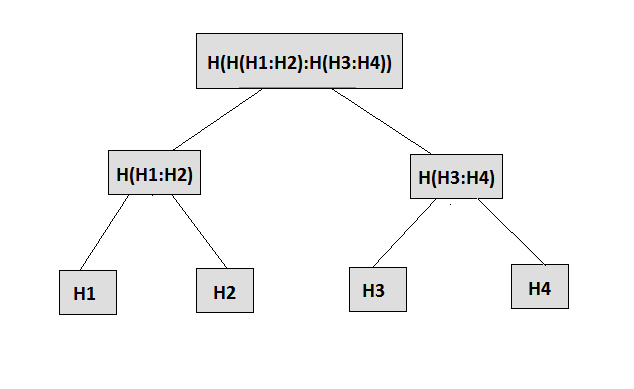
\includegraphics[width=0.8\textwidth]{Merkle_tree}
\end{figure}
    
\section{Radix Path Identifier}
An important requirement of the chosen PoDP scheme is to efficiently store, retrieve and re-evaluate the root hash value of the Merkle hash tree from the leaf hash values on every challenge request by the client. 

To encode, store and later decode and re-evaluate the Merkle hash tree, we have made use of the Radix Path Identifier  as proposed by Muhammad Saqib Niaz and Gunter Saake ~\cite{Paper13} in their paper, and  Vijay Atluri and Günther Pernul ~\cite{IntegrityBook} in their book. 

The basic idea of using Radix Path Identifier(RPI) is to assign a unique number to each node in the Merkle hash tree so that its level can clearly be identified and its parent node can be easily derived. In order to generate this unique number, radix or base value needs to be defined. For our implementation we defined the order of the generated tree (max nodes that can be contained in an internal node) to be used as the radix r\textsubscript{b}. Now if l is the level of a node and i is the index of a value within the node, RPI value of each node can be defined as explained below:      

\[
    rpi = 
\begin{dcases}
    \ l+i, & \text{if}\ l==0 \\
 	\ rpi_{parent} * r_{b} + i, & \text{if}\ l>0
\end{dcases}
\]

In order to better understand how it works, consider Figure 5.2. Assume that the file is divided into 6 blocks - indexed 1 to 6. These blocks are then inserted into the B+ tree of order 3. After all the blocks are inserted, the resultant tree has three levels as shown in the figure. After the tree is generated, the RPI is generated as per the formula above. For e.g., the root node(l = 0) RPI values will be 0, 1, 2 (= their respective indices). Note that all leaf nodes will always have index 0 and all the calculations done are based on ternary number system. Now consider block 5. As per the formula, its RPI is equal to RPI of its parent multiplied by radix, hence the value 200.

The two important requirements listed above to ensure re-evaluation of the root hash value are fulfilled by this scheme as follows:
\begin{itemize}
\item A node's parent RPI rpi\textsubscript{parent} can be calculated as rpi/r\textsubscript{b}
\item A node pointer's index can also be calculated using formula rpi mod r\textsubscript{b}  
\end{itemize}

Upon receiving individual block hashes from a cluster node, the remote server loads the hashes of remaining blocks and regenerates the root hash value moving from bottom to top. 
\begin{figure}[h]
\caption{ Radix path identifier for Merkle hash tree}
\centering
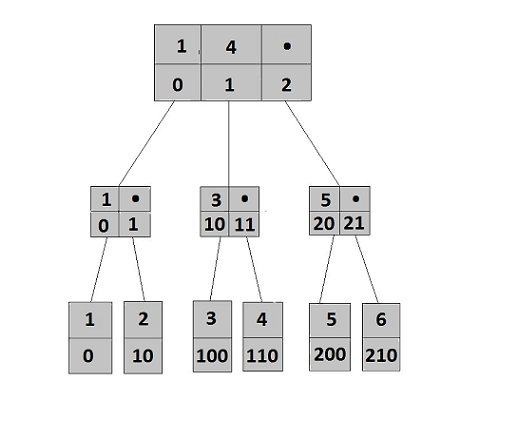
\includegraphics[width=0.8\textwidth]{rpi}
\end{figure}
     
\chapter{The Solution}
\label{cha:The Solution}
\section{General approach}
A Proof of Data Possession (PoDP) scheme involves an audit mechanism in which after the storage of his/her data on the cloud, the client can audit the cloud storage at any point of time and get a response with smallest amount of computation, time and network overhead to ensure that the cloud provider is still in possession of the data.\paragraph{}

Data integrity schemes can be divided into two main categories, i.e., probabilistic and deterministic.
Deterministic techniques ensure complete data possession by the storage system. These techniques are generally storage and computation heavy. 
As the name suggests, probabilistic techniques can only assure that there is a high likelihood of data possession by the storage system. Such schemes generally have lower storage and/or computation overheads, which make them preferred choice of PoDP mechanisms. Also, if probabilistic schemes are used repeatedly over time, they can ensure complete data possession.\paragraph{}

Based on these techniques, following possible mechanisms can be utilized. Their advantages and drawbacks have also been discussed:
\begin{itemize}
\item A possible solution could be that the client application retains the local copy of the data. The user then requests for the entire file data during challenge/audit phase from the cluster node and then compares the entire file with local file data.
Clearly, this is a deterministic theme which involves high storage overhead, thus defeating the purpose of data outsourcing.
\item Another possible solution could be a probabilistic scheme involving hash function. A hash function is a one-way mathematical function that maps a large sized data to a smaller fixed size hash value. Since they are irreversible, i.e., the data cannot be derived from its hash value and they generate a fairly compact code. Hash functions are widely used in multiple PoDP schemes. 

One commonly used scheme is to divide given file data into blocks of fixed size and generate hash values/tags for each block before transmitting the file to the cluster node. During audit, the cluster node is requested to return hash tags for given set of blocks, thus ensuring possession of that many blocks of data.

A problem with this technique is that the block size cannot be kept too large as it reduces the number of times an audit can be performed on the cluster node to ensure data possession. For example, if a file is broken into three blocks, the client can only audit the cluster three times after which, the cluster node could simply store all the hash codes previously requested and delete the file. On any subsequent audit, the cluster node can simply return the stored hash tag, thus making the audits useless. 

If the block size is kept very small, it would result in large number of tags to be stored at client's device, thus increasing the storage and network overhead of the algorithm. 

\item Another possible probabilistic technique using hash functions with smaller block sizes involves making use of Merkle hash trees. This technique could also reduce storage and network overhead .
A Merkle hash tree is a tree based cryptographic data structure in which the hash values/tags of each data block are at the leaves of the tree and every non-leaf node is labelled with the cryptographic hash of the labels of its child nodes. Hash trees allow efficient and secure verification of the contents of large data structures.
For example, in a simple binary hash tree with two leaves with Hash values(0-0) and (0-1), hash 0 would be the result of hashing the concatenation of hash 0-0 and hash 0-1. That is, hash 0 = hash( hash(0-0) + hash(0-1) ) where + denotes concatenation.

Though Merkle hash trees clearly have an advantage from storage and network bandwidth point of view (if only root hash is transmitted), they require higher computation requirements.

\item In order to reduce the load of computation in the client device, another proposed idea is to make use of a trusted server. It could be a third party server or the remote server within the cloud infrastructure that can bear the burden of computation and storage of Merkle hash tree related information and querying different cluster node replicas on each audit.
The cloud provider could provide this feature to increase trust in their platform. Also, they could embed these qualities in one of their cluster manager/server.
\end{itemize}

Since the usage of Merkle hash trees using a third-party or cloud remote server seems to be the most optimal solution in terms of computation, network and storage overhead, we chose this technique to implement it and test its performance.  
\section{Algorithm}

\section{Architecture}
The exchanges between the client, the remote server and the cluster nodes on cloud can generally be described as shown in Figure 4.1 below can be explained as follows:
\begin{figure}[h]
\caption{ 	}
\centering
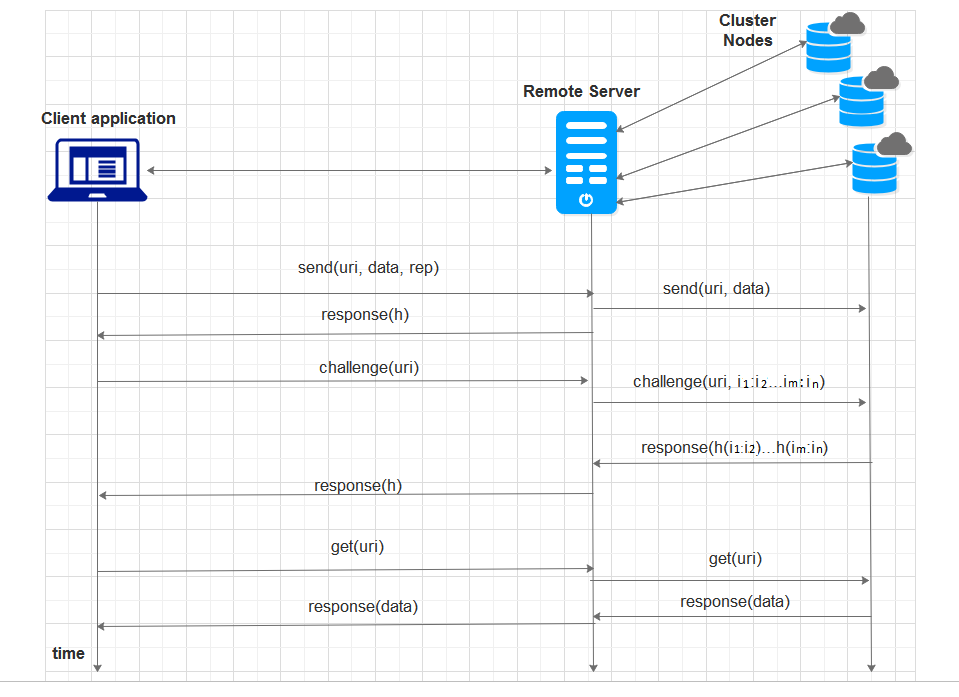
\includegraphics[width=0.8\textwidth]{architecture}
\end{figure}

\begin{enumerate}
\item \emph{send(url, replication count)}\newline
The client application on user's device sends a local file to be uploaded on cloud to a remote server.
On receiving the file, the remote server calculates the block size based on file size and generates the Merkle hash tree with hash values of each block. It then sends the file to the required number of cluster nodes based on replication count. 
On successfully saving the file on each replica, the remote server stores the Merkle hash tree and some metadata  (explained later) in its local database. It then sends the root hash value of the Merkle hash tree to the client application which then stores this root hash in user's device's local DB.
\item \emph{challenge(file)} \newline
At any later point, the client can query the remote server to generate the proof of data possession by some cluster node. The client can conduct such tests multiple times.

The remote server upon getting this request retrieves the Merkle hash tree and the metadata (like file size, block count, block size) for the file. It then randomly selects one of the cluster nodes and selects fifteen/twenty percent of blocks and sends the list of file indices(i\textsubscript{1}:i\textsubscript{2}...i\textsubscript{m}:i\textsubscript{n}) for which the cluster node should return hashes.
 
\item \emph{challenge(file, i\textsubscript{1}:i\textsubscript{2}...i\textsubscript{m}:i\textsubscript{n})} \newline
The cluster node on receiving this request fetches the file and generates a list of hashes for the indices and returns it as part of response to the remote server.

\item \emph{response(h\textsubscript{12}...h\textsubscript{mn})} \newline
The remote server on receiving the response, re-evaluates the Merkle hash tree root value by using the response hashes and hashes of remaining blocks (non-queried) from its local database and sends the response back to the client.

\item \emph{response(h)} \newline
The client on receiving the response verifies it against the hash value stored in its local store to get the PoDP by at least one of the cluster nodes. 

\end{enumerate}

\chapter{Implementation \& technical details}
The PoC for the proposed Proof of Data possession algorithm is implemented in C++ on Ubuntu platform. It comprises of the following important modules, each of which has been discussed in detail in further subsections:
\begin{enumerate}
\item A RESTful web server to receive and send files over HTTP.
\item A fast and efficient key-value database to store the Merkle hash tree.
\item Module to split the file into blocks and generate Merkle hash tree(B+ tree) for the file.
\item Module to retrieve and parse the Merkle hash tree and to generate root hash value of the Merkle tree using partial hash values returned from cluster-node and the remaining values from the database.
\end{enumerate}

\section{RESTful Server}
In order to implement the PoC, the first requirement is an appropriate multi-threaded RESTful framework. The framework needs to have a simple implementation for both client and a server providing functionality for standard APIs like POST, GET and custom API that can be extended to implement challenge/Response. Microsoft's cpprestsdk, Corvusoft's  restbed and Pistache were considered. Corvusoft's restbed was chosen as it has more flexible APIs with a relatively simple implementation. Since the framework is not an inherent part of the algorithm, it can be replaced with any other framework. However, the selected framework needs to provide following functionality.

The RestServer is configured to handle GET, POST and CHALLENGE methods and is then started with details about Cluster Nodes.  
\begin{verbatim}
one->set_method_handler( "POST", postMethodHandler );
two->set_method_handler( "GET", getMethodHandler);
three->set_method_handler( "CHALLENGE", challengeMethodHandler);
\end{verbatim}

On receiving a POST request, the server downloads the file, generates its Merkle hash tree, stores its encoded version in its local database and then sends the file to cluster-nodes based on replication. In order to generate the Merkle tree, the server determines the block size and block count  based on file size. It then generates hash values of each block, encodes them and add them to the leaf of the B+ Tree. 
The generated tree is then stored in the local key-value, the file then sent to the cluster node and the root hash value is then  returned to the client
\begin{verbatim}
int blocksize = getBlockSize(fileData.length());
string rootHash = generateBTree(fileName, fileData, blocksize, order);
session->close( OK, rootHash );
\end{verbatim} 
The generateBTree function has following functionality:   
\begin{verbatim}
while(remsz > 0) {
	root = btree->insert(root, blocknum, record);
	btree->evaluate(root);
	btree->generate_rpi(root);
	btree->dumpDataOnDB(mDB, filename.c_str(), root, blocksize, blocknum - 1);
}
\end{verbatim} 
On receiving a CHALLENGE request, the server retrieves and decodes the Merkle hash tree in its local database for the requested file. It then selects some random blocks and sends an array of start\_index:end\_index to the cluster node. 

\begin{verbatim}
rpiA->parse(mDB, body.c_str()/*file URI*/);
int cn_id = rand()%mSendFiles.size();
string response = mSendFiles[cn_id]->challenge(body.c_str(), params);
\end{verbatim}  

The server then feeds these responses to the algorithm to regenerate the root hash and return it to the client.

\begin{verbatim}
rpiA->validate(blocknums, hashes, chalRes);
session->close( OK, chalRes, { { "Content-Length", ::to_string( chalRes.size( ) ) } } );
\end{verbatim} 

In the next section, the generation, encoding, parsing and re-evaluation of the Merkle hash tree is discussed.
\section{Merkle B+ tree and Radix Path Identifier}
In order to generate the tree, a recursive top to bottom approach was used in which block hashes were first added to the root node and then subsequently the nodes are split when they are full. We adapted the B+ tree implementation by Amittai Aviram(which was written in C) and modified it based on the requirements mentioned above.
    
\section{Radix Path Identifier}
Once the Merkle hash tree has been generated by the server, it needs to store it in its local database until a challenge is received for the file. To do this, RPI is generated for each node of the MHT using a depth first approach. Later on receiving a challenge request,  receiving individual block hashes from a cluster node, the remote server loads the hashes of remaining blocks and regenerates the root hash value moving from bottom to top. 
 
\section{Key-value Datastore}
As previously mentioned, the Remote Server needs to store each file's  Merkle hash tree and some metadata. The metadata that is stored per file is required for validation. 
\begin{verbatim}
proot.put("levels", this->num_level + 1);
proot.put("blockcount", blockcount);
proot.put("blocksize", blocksize);
proot.put("order", this->order);
\end{verbatim}

The block-hashes with levels and the metadata stated above is encoded in json format. It needs to be stored in a key-value store. Redis DB and RocksDB are two such key-value stores that were considered to store this data. Since RocksDB is an embedded key/value store supporting multi-threaded persistence, it was preferred over Redis DB, which is a remote in-memory store (more suitable when data needs to be stored on another server).
\section{Safety measures}
The safety of this algorithm depends upon the strength of hash function used. We have used openssl's sha256  
\chapter{The Performance Impact}
\label{cha:The Performance Impact}
Performance impact of a PoDP scheme can be measured in terms of network overhead, storage overhead and computational overhead. Clearly, network and storage overhead of this algorithm is quite low. This is so because only hash values are exchanged apart from sending and retrieving file and the client device only needs to store the file URI and its 256 root hash value. 

The most important performance impact of this algorithm is the computational overhead thus causing time overhead during POST operation of the file. In order to account for this time overhead of the implemented PoDP scheme, we tested it on a cluster environment to imitate real life scenarios. It involved the client application, the remote server and one, two or three cluster nodes all running on their own different machines. The count of cluster nodes in each experiment defines the replication count for each file as chosen by client. 

The test was performed by taking an average of the time-lags recorded for each operation over two hundred times for different file sizes, also to mimic real world behaviour.
The numbers shown in each table and graph is the average value of each scenario of those two hundred runs.
Tests marked secured define the case where the remote server supports our algorithm of generating Merkle hash tree and supporting challenge function calls. Tests marked non-secured are cases where remote-server simple acts as a relay.
\section{Results}
As can be seen from Table 6.1, the generation and saving of MHT, RPI and metadata increases the overall response time by 0.01 second on an average irrespective of the file size. This effect can be also be seen in Figure 6.1, 6.2 and 6.3 respectively.  Though it seems like a large overhead for smaller files(64KB), the overhead is still well within reasonable range in order to enable security and trust in cloud users. Also, the time lag becomes negligible as the size of files increase.

The time overhead of challenge-response APIs was tested as well which is shown in Table 6.2. As expected, the time taken by this API is independent of file-size until files are not extremely large. This is because of the following reasons:
\begin{itemize}
\item On every challenge request, the remote server needs to load and parse RPI based Merkle hash tree and send a single to one of the cluster nodes.
\item On receiving a challenge request, a cluster node needs to load the file from its database and perform hash-functions and return results to the server.
\item In terms of data transmitted, only file URI, indices, hash values etc are sent over the network.
\end{itemize} 

  
\begin{table}[]
\caption{Send file time statistics(in seconds) for secured and non-secured mode}
\label{tab:my-table}
\begin{tabular}{@{}|l|l|l|l|l|l|l|l|@{}}
\toprule
\rowcolor{mediumgray} 
\textbf{S.No.} &
  \textbf{File size (KB)} &
  \multicolumn{2}{l|}{\cellcolor{mediumgray}\textbf{1 Cluster node}} &
  \multicolumn{2}{l|}{\cellcolor{mediumgray}\textbf{2 Cluster nodes}} &
  \multicolumn{2}{l|}{\cellcolor{mediumgray}\textbf{3 Cluster nodes}} \\ \midrule
\multicolumn{2}{|l|}{\textbf{}} &
  \cellcolor{lightgray}\textbf{Non-Secured} &
  \cellcolor{lightgray}\textbf{Secured} &
  \cellcolor{lightgray}\textbf{Non-Secured} &
  \cellcolor{lightgray}\textbf{Secured} &
  \cellcolor{lightgray}\textbf{Non-Secured} &
  \cellcolor{lightgray}\textbf{Secured} \\ \midrule
1 & 64   & 2.0358  & 2.0413  & 2.03665 & 2.04735 & 2.0383  & 2.05    \\ \midrule
2 & 128  & 2.041   & 2.04455 & 2.04145 & 2.04955 & 2.0437  & 2.0502  \\ \midrule
3 & 256  & 2.04985 & 2.05925 & 2.04995 & 2.06065 & 2.0507  & 2.06565 \\ \midrule
4 & 512  & 2.0681  & 2.07195 & 2.073   & 2.07325 & 2.07045 & 2.0766  \\ \midrule
5 & 1024 & 2.0997  & 2.1062  & 2.10175 & 2.1093 & 2.10955 & 2.11625 \\ \bottomrule
\end{tabular}
\end{table}

\begin{table}[]
\caption{Challenge function time statistics((in seconds)}
\label{tab:tablechallenge}
\begin{tabular}{@{}|l|l|l|l|l|@{}}
\toprule
\rowcolor{mediumgray} 
\textbf{S.No.} & \textbf{File size (KB)} & \textbf{1 Cluster node} & \textbf{2 Cluster nodes} & \textbf{3 Cluster nodes} \\ \midrule
1 & 64   & 0.0272  & 0.0276  & 0.0275  \\ \midrule
2 & 128  & 0.02735 & 0.02735 & 0.02765 \\ \midrule
3 & 256  & 0.0272  & 0.02765 & 0.02755 \\ \midrule
4 & 512  & 0.0269  & 0.02705 & 0.02765 \\ \midrule
5 & 1024 & 0.0273  & 0.02755 & 0.0274  \\ \bottomrule
\end{tabular}
\end{table}

\begin{figure}
\centering
    \begin{tikzpicture}[thick,scale=0.8, every node/.style={scale=0.8}]
      \begin{axis}[
        width=0.8\linewidth,
        ybar=0pt,
        bar width=7.5pt,
        ymin=2.03,
        enlarge x limits={abs=25pt},
        legend style={draw=none,at={(0.5,-0.15)}, text width=2.5cm,
        anchor=north,legend columns=-1},
        xlabel={File size(in KB)},
        ylabel={Time (in seconds)},
        x tick label style={/pgf/number format/1000 sep={}},
        xmajorgrids=true,
        cycle list={blueaccent, mediumgray},
        x tick label as interval,
      ]
        \pgfplotsinvokeforeach{Non-Secured, Secured}{
        \addplot+[draw=none, fill, area legend,] table [col sep=comma,x expr=\thisrow{File-Size}+0.5,y=#1]{\mytableonenode};
        \addlegendentry{#1}
        }
    \end{axis}
    \end{tikzpicture}
    \caption{Performance of secured Vs Non-secured file save on cloud with one cluster node}
    \label{fig:OneNode}
\end{figure}

\begin{figure}
\centering
    \begin{tikzpicture}[thick,scale=0.8, every node/.style={scale=0.8}]
      \begin{axis}[
        width=0.8\linewidth,
        ybar=0pt,
        bar width=7.5pt,
        ymin=2.03,
        enlarge x limits={abs=25pt},
        legend style={draw=none,at={(0.5,-0.15)}, text width=2.5cm,
        anchor=north,legend columns=-1},
        xlabel={File size},
        ylabel={Time (in seconds)},
        x tick label style={/pgf/number format/1000 sep={}},
        xmajorgrids=true,
        cycle list={blueaccent, mediumgray},
        x tick label as interval,
      ]
        \pgfplotsinvokeforeach{Non-Secured, Secured}{
        \addplot+[draw=none, fill, area legend,] table [col sep=comma,x expr=\thisrow{File-Size}+0.5,y=#1]{\mytabletwonodes};
        \addlegendentry{#1}
        }
    \end{axis}
    \end{tikzpicture}
    \caption{Performance of secured Vs Non-secured file save on cloud with two cluster nodes}
    \label{fig:OneNode}
\end{figure}

\begin{figure}
\centering
    \begin{tikzpicture}[thick,scale=0.8, every node/.style={scale=0.8}]
      \begin{axis}[
        width=0.8\linewidth,
        ybar=0pt,
        bar width=7.5pt,
        ymin=2.03,
        enlarge x limits={abs=25pt},
        legend style={draw=none,at={(0.5,-0.15)}, text width=2.5cm,
        anchor=north,legend columns=-1},
        xlabel={File size (in KB)},
        ylabel={Time (in seconds)},
        x tick label style={/pgf/number format/1000 sep={}},
        xmajorgrids=true,
        cycle list={blueaccent, mediumgray},
        x tick label as interval,
      ]
        \pgfplotsinvokeforeach{Non-Secured, Secured}{
        \addplot+[draw=none, fill, area legend,] table [col sep=comma,x expr=\thisrow{File-Size}+0.5,y=#1]{\mytablethreenodes};
        \addlegendentry{#1}
        }
    \end{axis}
    \end{tikzpicture}
    \caption{Performance of secured Vs Non-secured file save on cloud with three cluster nodes}
    \label{fig:OneNode}
\end{figure}

\chapter{Conclusion and Future Work}
\label{cha:Conclusion and Future Work}
As can be seen from the experiments, the proposed scheme for PoDP is quite efficient with minimal performance overhead. So it can be concluded that this algorithm can be used by cloud-providers to assure its users of their data-possession. If on each challenge request, the remote server queries each of replica in the cluster, it could be a scheme for Proof of Data Replication.
\section{Future work}
Intel Software Guard Extensions (SGX) is a set of security-related instruction codes that are built into some modern Intel central processing units (CPUs). They allow user-level as well as operating system code to define private regions of memory, called enclaves, whose contents are protected and unable to be either read or saved by any process outside the enclave itself, including processes running at higher privilege levels.

As can be seen, this scheme heavily relies on a cloud or third-party trusted server to perform computations. In order to reduce chances of infiltrations in these servers,in the future, the operations like Merkle hash tree and RPI generation and re-evalution of root hash-values can be done in secured enclaves. The implementation was done modularly so that only required code can be executed in such enclaves.

\chapter{Acknowledgement}
I would like to sincerely thank my guide Prof. Dr. Pascal Felber for offering me the chance to research and implement such a challenging and exciting topic for my Master’s thesis. I also wish to express my immense gratitude to my supervisor Prof. Dr. Valerio Schavioni who made it possible for me to complete this work. During the entire duration of the project, he provided me with continuous motivation, resources to guide me in my research and constant feedback to make improvements in work. 


On the personal front, I would like to thank my son Ayaan, who was born in the midst of project duration, who inspired me to finish this work. I am also indebted to my family and work colleagues who provided my with support whenever I needed. Finally, I would like to dedicate this thesis to my husband, Prakash who provided me with support and motivation and without whom this could not have been possible.
\bibliography{thesis}
\bibliographystyle{plain}
\begin{thebibliography}{1}
\bibitem{PDPDef}
Authors: Shuai Han, Shengli Liu, Kefei Chen, Dawu Gu
Article: Proofs of Data Possession and Retrievability
Based on MRD Codes
Link: https://eprint.iacr.org/2013/789.pdf
Other info: (retrieved October 2019).

\bibitem{JnK}
Authors: Ari Juels1 and Burton S. Kaliski Jr.2
Article: PORs: Proofs of Retrievability for Large Files
Link:https://www.arijuels.com/wp-content/uploads/2013/09/JK07.pdf
Other info: (retrieved December 2019)
\bibitem{GRRJ}
Authors: Giuseppe Ateniese, Randal Burns, Reza Curtmola,
Joseph Herring, Lea Kissner, Zachary Peterson, Dawn Song
Article: Provable Data Possession at Untrusted Stores
Link: https://eprint.iacr.org/2007/202.pdf
Other info: (retrieved October 2019).

\bibitem{DPS}
Authors: Décio Luiz Gazzoni Filho, Paulo Sérgio Licciardi Messeder Barreto
Article: PORs: Proofs of Retrievability for Large Files
Link:https://www.arijuels.com/wp-content/uploads/2013/09/JK07.pdf
Other info: (retrieved December 2019)

\bibitem{YJA}
Authors: Yves Deswarte, Jean-Jacques Quisquater, Ayda Saïdane
Article: Remote Integrity Checking
Link: https://link.springer.com/content/pdf/10.1007%2F1-4020-7901-X_1.pdf
Other info: (retrieved October 2019).


\bibitem{Paper13}
Authors: Muhammad Saqib Niaz, Gunter Saake 
Article: Merkle Hash Tree based Techniques for Data Integrity of Outsourced Data
Link: http://ceur-ws.org/Vol-1366/paper13.pdf
Other info: (retrieved June 2016).

\bibitem{}
Authors: Hovav Shacham, Brent Waters
Article: Compact Proofs of Retrievability
Link: https://hovav.net/ucsd/dist/verstore.pdf
Other info: (retrieved January 2020).

\bibitem{MHT}
Site: Merkle hash trees
Link: https://en.wikipedia.org/wiki/Merkle\_tree
Other info: (retrieved January 2020).

\bibitem{RestSdk}
Site: A Microsoft C++ REST SDK
Link: https://github.com/microsoft/cpprestsdk
Other info: (retrieved January 2020).

\bibitem{Pistache}
Site: An elegant purely C++11 REST framework
Link: http://pistache.io/
Other info: (retrieved January 2020).

\bibitem{Restbed}
Site: Corvusoft's Restbed framework brings asynchronous RESTful functionality to C++11 applications
Link: https://github.com/Corvusoft/restbed
Other info: (retrieved January 2020).

\bibitem{RocksDB}
Site: An embeddable persistent key-value store for fast storage
Link: https://rocksdb.org/
Other info: (retrieved June 2016).


\bibitem{BPlusTree}
Author:Amittai Aviram
Site: B+ Tree C Implementation
Link: http://www.amittai.com
Other info: (retrieved January 2020).

\bibitem{IntegrityBook}
Authors: Vijay Atluri, Günther Pernul  
Article: Integrity Assurance for Outsourced Databases without DBMS modification
Book: Data and Applications Security and Privacy XXVIII: 28th Annual IFIP WG 11.3 Working Conference, DBSec 2014, Vienna, Austria, July 14-16, 2014, Proceedings (Lecture Notes in Computer Science) 2014th Edition 

\bibitem{SHA}
Site: SHA-2
Link: https://en.wikipedia.org/wiki/SHA-2
Other info: (retrieved January 2020).

\bibitem{SGX}
Site: Software Gaurd Extensions
Link: https://en.wikipedia.org/wiki/Software\_Guard\_Extensions
Other info: (retrieved January 2020).

\bibitem{PoRHardness}
Authors : Dodis, Yevgeniy and Vadhan, Salil and Wichs, Daniel
title : Proofs of Retrievability via Hardness Amplification Theory of Cryptography
Link : https://dl.acm.org/doi/10.1007/978-3-642-00457-5\_8
Other info: (retrieved January 2019)

\end{thebibliography}


%END Doc
%-------------------------------------------------------
\end{document}
